\documentclass{article}
\usepackage{graphicx}
\usepackage{amsmath}
\usepackage{listings}
\usepackage{xcolor}
\usepackage{hyperref}
\usepackage{color}
\definecolor{keywordcolor}{rgb}{0.8,0.1,0.5}
\definecolor{webgreen}{rgb}{0,.5,0}
\title{License Plate Recognition Algorithm Explanation Document}
\author{}
\date{}
\lstset{
	% 进行参数设置
	language=Java, % 设置语言
	basicstyle=\ttfamily, % 设置字体族
	breaklines=true, % 自动换行
	keywordstyle=\bfseries\color{NavyBlue}, % 设置关键字为粗体,颜色为 NavyBlue
	morekeywords={}, % 设置更多的关键字,用逗号分隔	
	emph={self}, % 指定强调词,如果有多个,用逗号隔开
	emphstyle=\bfseries\color{Rhodamine}, % 强调词样式设置
	commentstyle=\itshape\color{black!50!white}, % 设置注释样式,斜体,浅灰色
	stringstyle=\bfseries\color{PineGreen!90!black}, % 设置字符串样式
	columns=flexible,
	numbers=left, % 显示行号在左边
	numbersep=2em, % 设置行号的具体位置
	numberstyle=\footnotesize, % 缩小行号
	frame=single, % 边框
	framesep=1em % 设置边框与代码的距离
	% Java代码
}
\begin{document}
	
	\maketitle
	
	\section{Image Channel}
	In OpenCV, images can be represented as channels 1, 2, 3, and 4, respectively:
	\begin{itemize}
		\item Channel 1 is a grayscale image;
		\item The 2-channel images are RGB555 and RGB565. The 2-channel diagram may be used in program processing, such as Fourier transform, where one channel is a real number and the other is an imaginary number, mainly for ease of programming. RGB555 is 16 bits, 2 bytes, 5+6+5. The first 5 bits of the first byte are R, the last 3 bits plus the second byte are G, and the last 5 bits of the second byte are B. It can be seen that the original image has been compressed;
		\item 3-channel color image (RGB);
		\item 4 channels are RGBA, which is RGB plus an A channel, also known as the alpha channel, representing transparency. PNG images are a typical type of 4-channel image. The alpha channel can be assigned values from 0 to 1 or from 0 to 255, indicating transparency to opacity.
	\end{itemize}
	
	\subsection{CvType Type Constant Combination Rules}
	\begin{itemize}
		\item Byte: number of bits, digits. There are 8 bytes, 16 bytes, 32 bytes, and 64 bytes. In Mat, the space occupied by each pixel is 8 bits, which is CV\_8.
		\item U|S|F :
		\begin{itemize}
			\item U: unsigned int, unsigned integer;
			\item S: signed int, signed integer;
			\item F: float, single precision floating-point type, float type itself has a sign. The terms signed and unsigned here refer to the binary encoding of images. In the process of writing, I mostly use unsigned symbols, namely CV\_8U and CV\_16U, when there is calculation involved.
			\item C [channels]: The number of channels in an image.
		\end{itemize}
		\textbf{For example, CV\_8UC3 is an 8-bit unsigned 3-channel (RGB color) image.}
	\end{itemize}
	
	\section{Grayscale Image}
	\begin{itemize}
		\item Color images usually include three components: R, G, and B. Grayscale conversion is the process of making the R, G, and B components of a color image equal.
		\item Each pixel in a grayscale image has only one sample color, and its grayscale is a multi-level color depth located between black and white.
		\item Pixels with higher grayscale values are brighter, while those with lower grayscale values are darker. The maximum pixel value is 255 (representing white) and the minimum pixel value is 0 (representing black).
	\end{itemize}
	\begin{lstlisting}[language=Java]
		Imgproc.cvtColor(inMat, dst, Imgproc.COLOR_BGR2GRAY);
	\end{lstlisting}
	
	\url{https://leejason.blog.csdn.net/article/details/106416128}
	
	\section{Image Filtering (Noise Reduction)}
	Image filtering, which suppresses the noise of the target image while preserving its detailed features as much as possible, is an indispensable operation in image preprocessing. The quality of its processing effect will directly affect the effectiveness and reliability of subsequent image processing and analysis. There are two types of purposes: one is vague; another type is to eliminate noise.
	
	\subsection{Gaussian Filtering}
	Also known as Gaussian blur, the principle of blur:
	\begin{itemize}
		\item Take a matrix (3x3, 5x5) and convolve it with the original image from left to right and top to bottom. Finally, assign the convolution value to the center pixel of the current convolution.
		\item The size and value of a matrix are commonly referred to as convolution kernels.
		\item Used to suppress noise, smooth images, and prevent detecting noise as edges.
		\item Compared to mean filtering, Gaussian filtering has a smaller degree of blur in images.
	\end{itemize}
	\begin{lstlisting}[language=Java]
		public static final int BLUR_KERNEL=3; //The size of the filtering kernel must be a positive odd number
		public static void gaussianBlur(Mat inMat, Mat dst) {
			Size ksize=new Size(BLUR_KERNEL, BLUR_KERNEL); //3x3
			Imgproc.GaussianBlur(inMat, dst, ksize, 0, 0, Core.BORDER_DEFAULT);
		}
	\end{lstlisting}
	
	\url{https://blog.csdn.net/qq_35294564/article/details/81142524}
	
	\subsection{Median Filtering}
	Replacing the grayscale value of a pixel with the median grayscale value in the pixel domain means replacing all values with the median value of a region. Can exclude the maximum and minimum values:
	\begin{itemize}
		\item Removing speckle noise and salt and pepper noise is very useful. Mean filtering noise is also involved in the operation.
		\item The median filtering time is more than 5 times that of the mean filtering.
	\end{itemize}
	\begin{lstlisting}[language=Java]
		public static final int BLUR_KERNEL=3; //The size of the filtering kernel must be a positive odd number
		public static void medianBlur(Mat inMat, Mat dst) {
			Size ksize = new Size(BLUR_KERNEL, BLUR_KERNEL); //3x3
			Imgproc.MedianBlur(inMat, dst, ksize, 0, 0, Core.BORDER_DEFAULT);
		}
	\end{lstlisting}
	
	\subsection{Mean Filtering}
	The mean filtering itself has inherent flaws, that is, it cannot protect image details well, and at the same time, it destroys the details of the image while denoising, making the image blurry and unable to remove noise points well, especially the salt and pepper noise.
	\begin{lstlisting}[language=Java]
		public static final int BLUR_KERNEL=5; //The size of the filtering kernel must be a positive odd number
		public static void blur(Mat inMat, Mat dst) {
			Point anchor = new Point(-1,-1);
			Size ksize = new Size(BLUR_KERNEL, BLUR_KERNEL);
			Imgproc.blur(inMat, dst, ksize, anchor, Core.BORDER_DEFAULT);
		}
	\end{lstlisting}
	
	\section{Affine Transformation}
	The general operations for changing images include zooming in, zooming out, rotating, etc., collectively referred to as \textbf{geometric transformations}; The main image transformations include affine transformation, projection transformation, and polar coordinate transformation.
	
	There are two main steps in transforming an image:
	\begin{itemize}
		\item Implementing the transformation of spatial coordinates means moving the image from its initial position to its final position.
		\item Use an interpolation algorithm to complete the grayscale value of each pixel in the output image.
	\end{itemize}
	INTER-NEAREST nearest neighbor interpolation;
	INTER\_LINEAR bilinear interpolation (default);
	When using pixel region relationships for resampling, downsampling, and image reduction in INTER\_AREA, it is used;
	INTER\_CUBIC 4x4 pixel neighborhood bicubic interpolation (used when enlarging images);
	Lanczos interpolation of INTER\_LANCZOS4 8x8 pixel neighborhood.
	
	\subsection{Translate}
	Translation is the simplest affine transformation; If the spatial coordinates (x, y) are moved 100 along the x-axis and 200 along the y-axis. The translated coordinates are (x+100, y+200).
	
	After generalizing this process, assume that any spatial coordinate (x, y) is first translated along the x-axis by Px and then along the y-axis by Py. The obtained coordinates are (x+Px, y+Py). The translation process can be represented by a matrix as follows:
	
	\begin{center}
		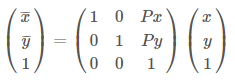
\includegraphics[width=0.5\textwidth]{mdpic/20240918163045.png}
	\end{center}
	
	Namely: \( dst=A \cdot inMat \) where A is an affine matrix.
	\begin{lstlisting}[language=Java]
		/**
		*@ param pX moves pixels horizontally; If it is greater than 0, it indicates positive movement along the axis; if it is less than 0, it indicates negative movement along the axis
		*@ param pY moves pixels vertically; If it is greater than 0, it indicates positive movement along the axis; if it is less than 0, it indicates negative movement along the axis
		*/
		public static void translateImg(Mat inMat, Mat dst, int pX, int pY) {
			//Define a translation matrix to create a fully zero matrix with 2 rows and 3 columns;
			//Normally, it should be 3 \times 3, but the value of the last line has been fixed to 0 0 1
			Mat trans_mat = Mat.zeros(2, 3, CvType.CV_32FC1);
			trans_mat.put(0, 0, 1);
			trans_mat.put(0, 2, pX);
			trans_mat.put(1, 1, 1);
			trans_mat.put(1, 2, pY);
			// Perform affine transformation using the translation matrix
			Imgproc.warpAffine(inMat, dst, trans_mat, inMat.size());
			}
		\end{lstlisting}
	
\subsection{Rotate}
To rotate an image around a specific center point, a rotation matrix can be created. The formula for rotation is as follows:

\[
\begin{bmatrix}
x' \\
y'
\end{bmatrix}
=
\begin{bmatrix}
\cos(\theta) & -\sin(\theta) \\
\sin(\theta) & \cos(\theta)
\end{bmatrix}
\begin{bmatrix}
x \\
y
\end{bmatrix}
\]

Where \((x', y')\) are the new coordinates after rotation and \(\theta\) is the rotation angle. The center of rotation can be specified to avoid shifting the image out of bounds.

\begin{lstlisting}[language=Java]
public static void rotateImg(Mat inMat, Mat dst, double angle, Point center) {
// Calculate the rotation matrix
Mat rot_mat = Imgproc.getRotationMatrix2D(center, angle, 1.0);
// Perform affine transformation using the rotation matrix
Imgproc.warpAffine(inMat, dst, rot_mat, inMat.size());
}
\end{lstlisting}

\subsection{Scale}
Scaling an image can either enlarge or shrink it. The scale factor determines the extent of this transformation.

\begin{lstlisting}[language=Java]
public static void scaleImg(Mat inMat, Mat dst, double scaleX, double scaleY) {
// Scaling the image using resize method
Imgproc.resize(inMat, dst, new Size(inMat.width() * scaleX, inMat.height() * scaleY));
}
\end{lstlisting}

\section{Conclusion}
In this document, we discussed various fundamental concepts related to image processing, including color channels, grayscale conversion, image filtering techniques, and affine transformations. Each method plays a crucial role in preparing images for further analysis, particularly in applications such as license plate recognition. Mastering these techniques is essential for effective image preprocessing and enhances the reliability of recognition algorithms.

\end{document}